\chapter{Nomes das Funcionalidades}
\label{detalhes:altera-nomes}

% \newcommand{\sepCapaProjeto}{Projeto Sistema ASSEL}
% \newcommand{\sepCapaTipo}{\textsc{Nota Técnica}}
% \newcommand{\sepCapaTitulo}{Alterações nos Nomes 
	
%	de Funcionalidades}
% \newcommand{\sepCapaData}{22 de Setembro de 2022}
% \newcommand{\sepCapaVersao}{V1}
% \newcommand{\sepCapaFile}{sep-capa-rosa.pdf}
% \newcommand{\sepCapaCor}{pink}

\section{Tabela De-Para}

Usar como referência a seguinte tabela \ref{tab:altera-nomes:depara} que contém os nomes originais (até a versão 4.1.2 do Sistema ASSEL) das funcionalidades na coluna ``De'' e informa quais deverão ser os novos nomes dessas funcionalidades na coluna ``Para'':

\begin{table}[!h]
	\begin{center}
		\begin{tabular}{|c|c|}
			\hline
			\rowcolor{corCOULD!40} \multicolumn{2}{|c|}{\Large Nomes das Funcionalidades \normalsize} \\ \hline
			\rowcolor{corCOULD!40} \multicolumn{2}{|c|}{\Large Tabela ``De-Para'' de Alterações \normalsize} \\ 
			\rowcolor{corCOULD!40} \multicolumn{2}{|c|}{\large (Funcionalidades da Barra Lateral do Sistema) \normalsize} \\ \hline

			% CABEÇALHO        
			\rowcolor{lightgray}\textbf{De} & \textbf{Para} \\ \hline
			% CONTEÚDO
			% Código escrito manualmente
			\rowcolor{cldfC1!40} \cellcolor{corCOULD!10} Gerenciar Perfil & Administrar Perfis  \\ \hline
			\rowcolor{cldfC1!40} \cellcolor{corCOULD!10} Gerenciar Usuário & Administrar Usuários  \\ \hline
			\rowcolor{cldfC1!40} \cellcolor{corCOULD!10} Gerenciar Unidade & Administrar Unidades  \\ \hline
			\rowcolor{cldfC1!40} \cellcolor{corCOULD!10} Gerenciar e Analisar Ordem de Serviço & Gerenciar e Analisar Solicitações  \\ \hline
		\end{tabular}    
		\caption{\label{tab:altera-nomes:depara} Tabela ``de-para'' de alterações nos nomes das funcionalidades}
	\end{center}
\end{table}

\textbf{Observação:}
A funcionalidade ``Solicitar Ordem de Serviço'' permanece com o mesmo nome.

%\toGil{Confirmar com Gilberto} Confirmado na reuniao do dia 19/09/2022

\section{As alterações devem ocorrer:}


\subsection{Na barra lateral do sistema}

	Os nomes das funcionalidade da barra lateral do sistema devem ser alteradas:
		
	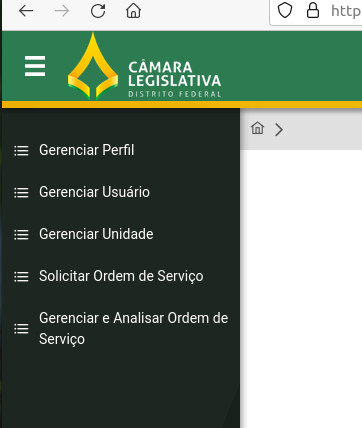
\includegraphics[width=0.8\textwidth]{fig/detalhes/barra-lateral.png}
	

\subsection{No texto das ``funcionalidades''}

	As funcionalidades da tela ``Gerenciar Perfis'' (que será renomeada para ``Administrar Perfis'') devem ser alteradas também:


	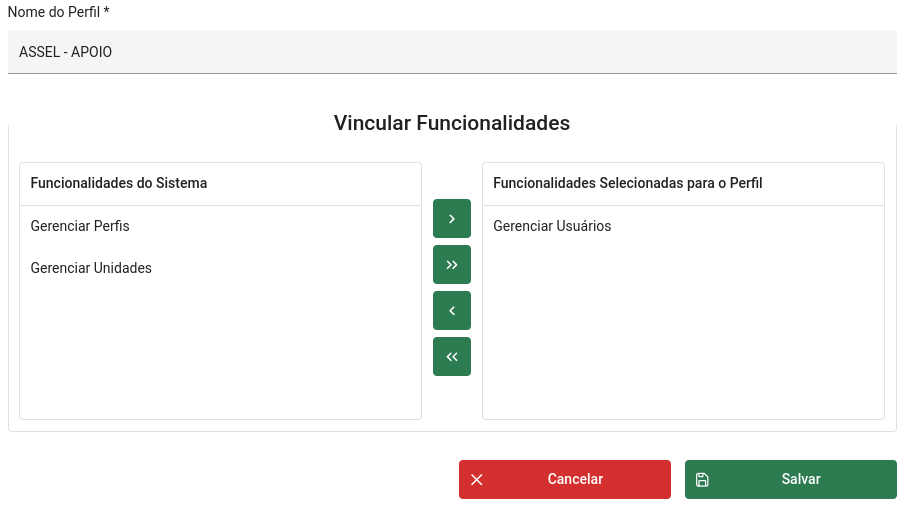
\includegraphics[width=0.8\textwidth]{fig/detalhes/vincular-funcionalidades.png}
	
\subsection{Quaisquer outros lugares}

	Quaisquer outros lugares no sistema onde essas funcionalidades aparecem devem ter seus nomes alterados de acordo.  
	
	
	\begin{center}
		\Large
		\textbf{FINAL DO DOCUMENTO}
		\normalsize
	\end{center}
	
